\documentclass{beamer}
\usepackage{graphicx}
\usepackage{verbatim}

\usetheme{Boadilla}

\title{The KS test}

\begin{document}

\frame{\titlepage}

\section{KS test}

\frame{
\frametitle{The KS Test}
\begin{itemize}
\item The KS test is a non-parametric test of the equality of two distributions
\begin{itemize}
\item The one sample KS test compares an empirical distribution to a known reference distribution
\item The two sample KS test compares the empirical distributions of two samples
\end{itemize}
\item The null hypothesis is that the two distributions are the same, in the two sample case, or that the sample is drawn from the reference distribution in the one sample case.
\end{itemize}
}


\section{The One Sample KS Test}

\frame{
\frametitle{The Empirical Cumulative Distribution Function}
For a random sample from the distribution $F_X$, the \emph{empirical cumulative distribution function} (ecdf), denoted $S_n(x)$, is defined as:
\[ S_n(x) = \frac{\text{number of sample values }\le x}{n} \]
In words, this is the proportion of sample values less than or equal to the specified value of $x$.
}

\frame{
\frametitle{The Empirical Cumulative Distribution Function}
\texttt{rvars = rnorm(25, mean = 0, sd = 1) \\
plot(ecdf(rvars), verticals = TRUE, do.points = FALSE)}
\begin{center}
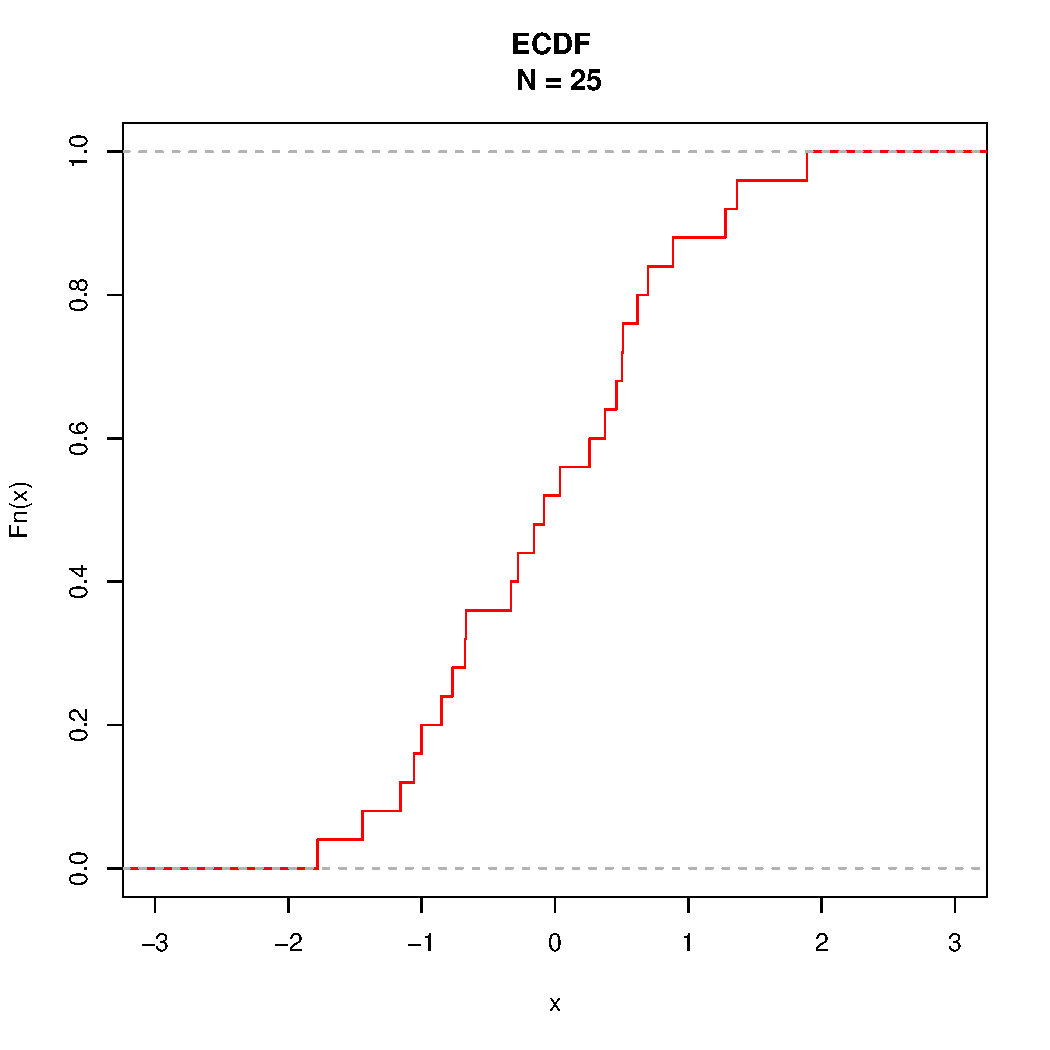
\includegraphics[scale = 0.35]{ex1.pdf}
\end{center}
}

\frame{
\frametitle{The One Sample KS Test}
The one-sample KS statistic is based on the difference between the hypothesized cumulative distribution function $F_0(x)$ and the empirical distribution function of the sample $S_n(x)$.
\begin{itemize}
\item The empirical distribution function $S_n(x)$ is a consistent estimate of the population cdf.
\item As $n$ increases, the step function $S_n(x)$, with jumps at the value of the sample order statistics $X_{(1)}, X_{(2)}, \dots, X_{(n)}$ approaches the true distribution $F_X(x)$ for all $x$
\end{itemize}
This implies that for large $n$, the deviations between the ecdf and the cdf, defined as $ | S_n(x) - F_X(x) |$ should be small.
Therefore, the \textbf{Kolmogorov-Smirnov one sample statistic is defined as:}
\[ D_n = sup_x | S_n(x) - F_X(x) | \]
}

\frame{
\frametitle{Example: One Sample KS against Normal}
\begin{center}
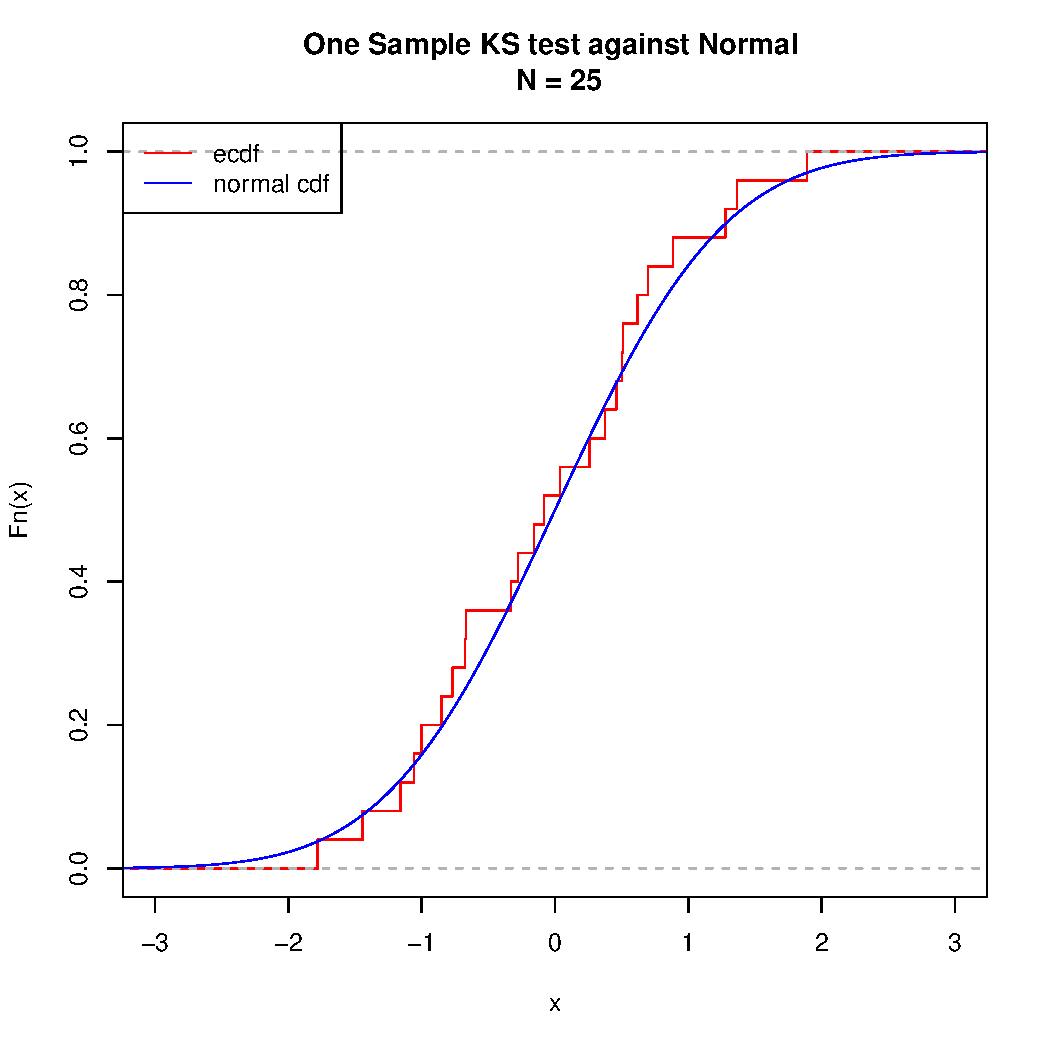
\includegraphics[scale = 0.2]{ex1b.pdf}
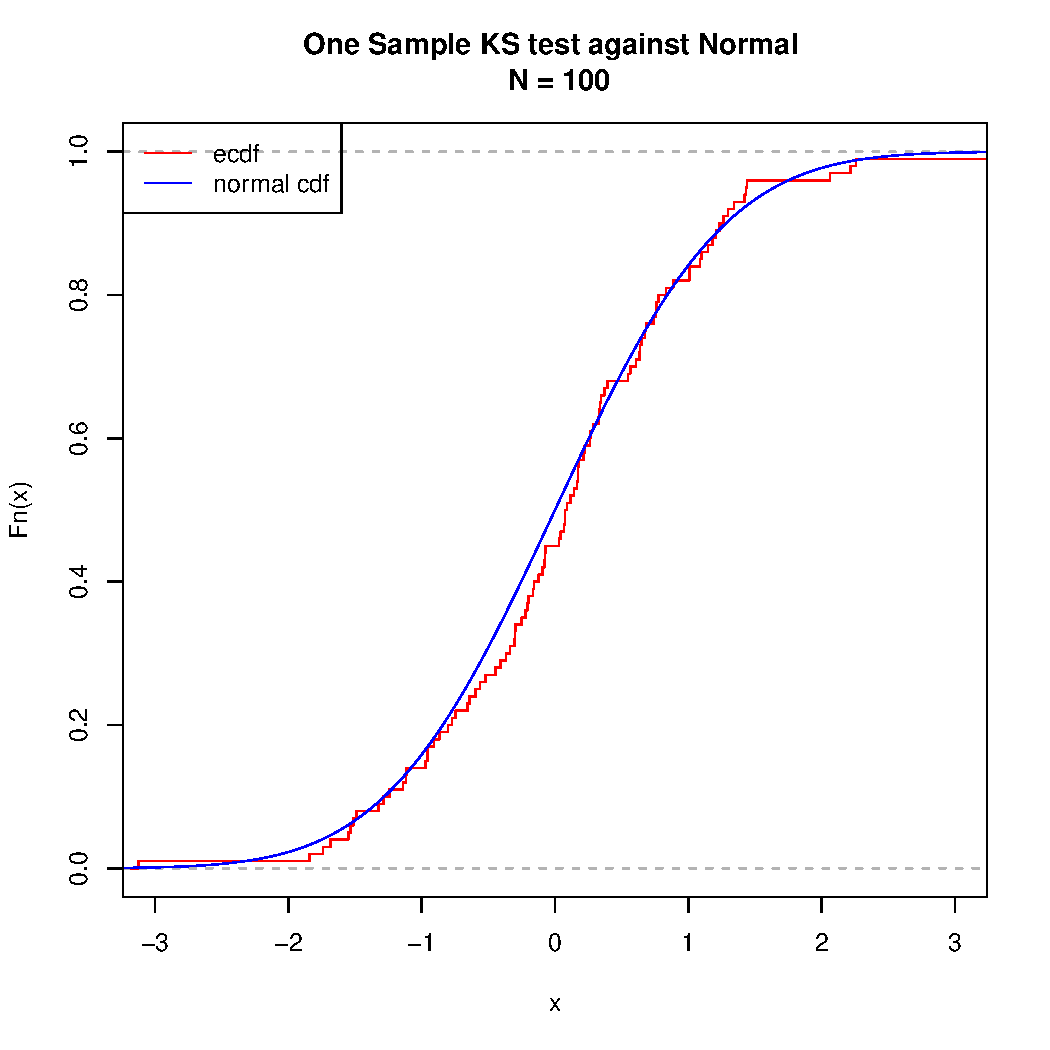
\includegraphics[scale = 0.2]{ex1c.pdf}
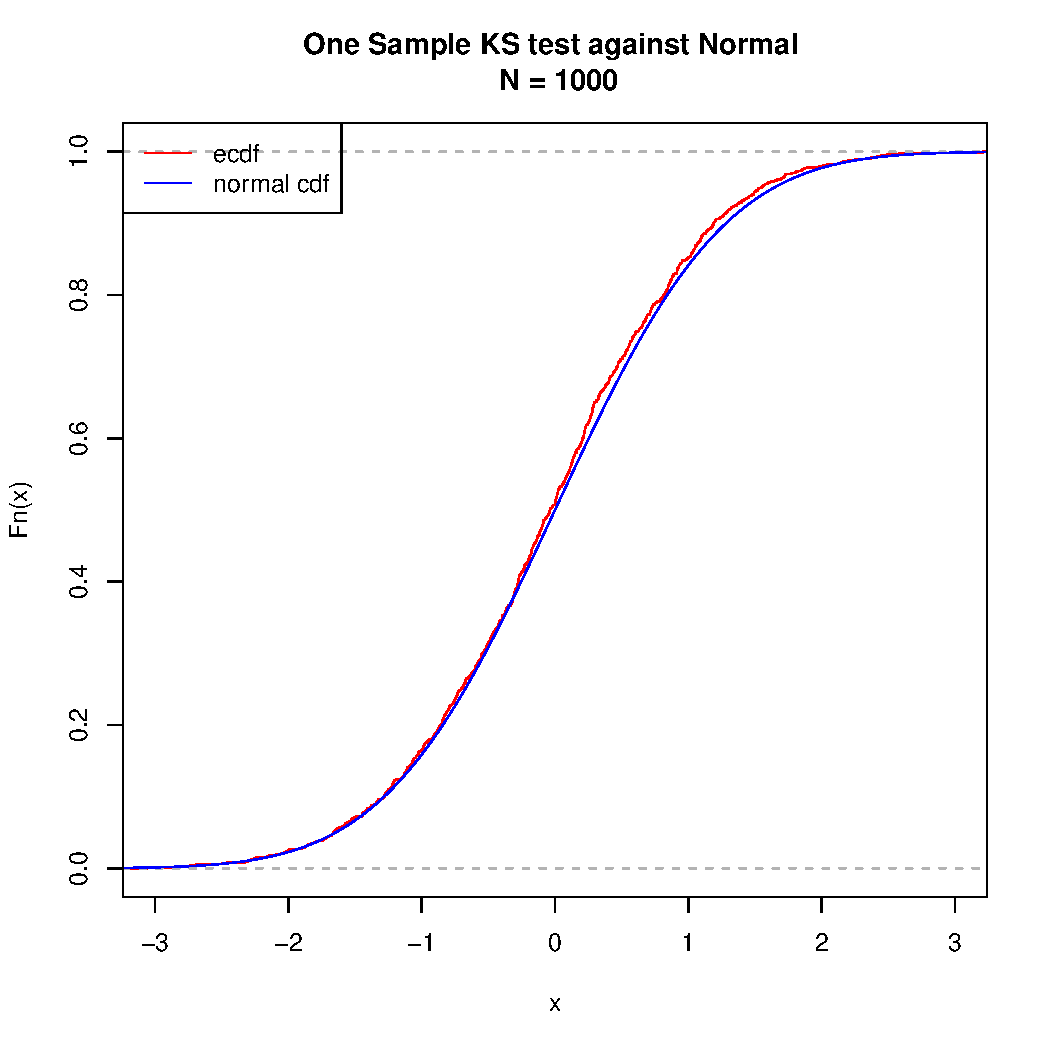
\includegraphics[scale = 0.2]{ex1d.pdf}\\
D = 0.1076806 $\qquad$
D = 0.07111517 $\qquad$
D = 0.03424409
\end{center}
where we use the call

\texttt{ks.test( x = rvars, y = pnorm)\$statistic}

to find the test statistics and

\texttt{ks.test( x = rvars, y = pnorm)\$p.value}

to find the p value
}

\frame {
\frametitle{Two-Sample Kolmogorov-Smirnov Test}

Define the order statistics of two samples of size $m$ and $n$ taken from populations $F_X$ and $F_Y$, repsectively, as:
\[ X_{(1)}, X_{(2)}, \dots, X_{(n)} \]
\[ Y_{(1)}, Y_{(2)}, \dots, Y_{(n)} \]

We can then define their respective empirical distribution functions as:
\begin{equation*} S_m(x) = \left\{
\begin{array}{rl} 0 & \text{if } x < X_{(1)}\\
\frac{k}{m} & \text{if } X_{(k)} < x < X_{(k + 1)}\\
1 & \text{if } x \ge X_{(m)} \end{array} \right.
\end{equation*}

\begin{equation*} S_n(x) = \left\{
\begin{array}{rl} 0 & \text{if } x < Y_{(1)}\\
\frac{k}{n} & \text{if } Y_{(k)} < x < Y_{(k + 1)}\\
1 & \text{if } x \ge Y_{(m)} \end{array} \right.
\end{equation*}
when we combine the total number of observations $n + m$ into a single sample, $S_m(x)$ and $S_n(x)$ are the proportions of $X$ and $Y$ observations which do not exceed the vale $x$, respectively.
}

\frame{
\frametitle{The Null for A Two-Sample Test}
The null hypothesis is that the two samples are coming from the same distribution:
\[ H_0: F_{Y(x)} = F_{X(x)} \qquad \text{ for all } x \]
\begin{itemize}
\item Because the edf for the $X$ and $Y$ samples are consistent estimates of the respective cdfs under $H_0$, we should observe that $S_m(x)$ and $S_n(x)$ are very similar.
\item The KS test defines ``similar'' as the maximum absolute difference between the two empirical distributions, $D_{n,m}$ as the metric of agreement.
\item $D_{n,m}$ is defined as
\[ D_{n,m} = sup_x|S_m(x) - S_n(x)| \]
\item Note that the alternative hypothesis is two-sided due to absolute value sign
\[ H_1: F_{Y(x)} \ne F_{X(x)} \qquad \text{ for some } x \]
\end{itemize}
}

\frame{

\frametitle{Example: Two Sample KS test}
\begin{itemize}
\item This is an example from \texttt{ http://www.physics.csbsju.edu/stats/KS-test.html}

\item Two near-by apple trees are in bloom in an otherwise empty field. One is a Whitney Crab the other is a Redwell. Do bees prefer one tree to the other? We collect data by using a stop watch to time how long a bee stays near a particular tree. We begin to time when the bee touches the tree; we stop timing when the bee is more than a meter from the tree. We wanted to time exactly the same number of bees for each tree, but it started to rain. Unequal dataset size is not a problem for the KS-test. 

\item This example is based on data distributed according to the Cauchy distribution: a particularly abnormal case.
\end{itemize}
}

\frame{
\frametitle{Example: Two Sample KS test}
\texttt{length(redwell) \# 80}\\
\texttt{length(whitney) \# 79}\\
\texttt{mean(redwell) \# 21.40275}\\
\texttt{mean(whitney) \# 21.11266}\\
\texttt{t.test(redwell, whitney)}\\
\texttt{	Welch Two Sample t-test}\\
\texttt{data:  redwell and whitney }\\
\texttt{t = 0.2057, df = 153.276, p-value = 0.8373}\\
\texttt{alternative hypothesis: true difference in means is not equal to 0 }\\
\texttt{95 percent confidence interval:}\\
\texttt{ -2.496598  3.076781 }\\
\texttt{sample estimates:}\\
\texttt{mean of x mean of y }\\
\texttt{ 21.40275  21.11266 }
}


\frame{
\frametitle{Example: Two Sample KS test}
\begin{center}
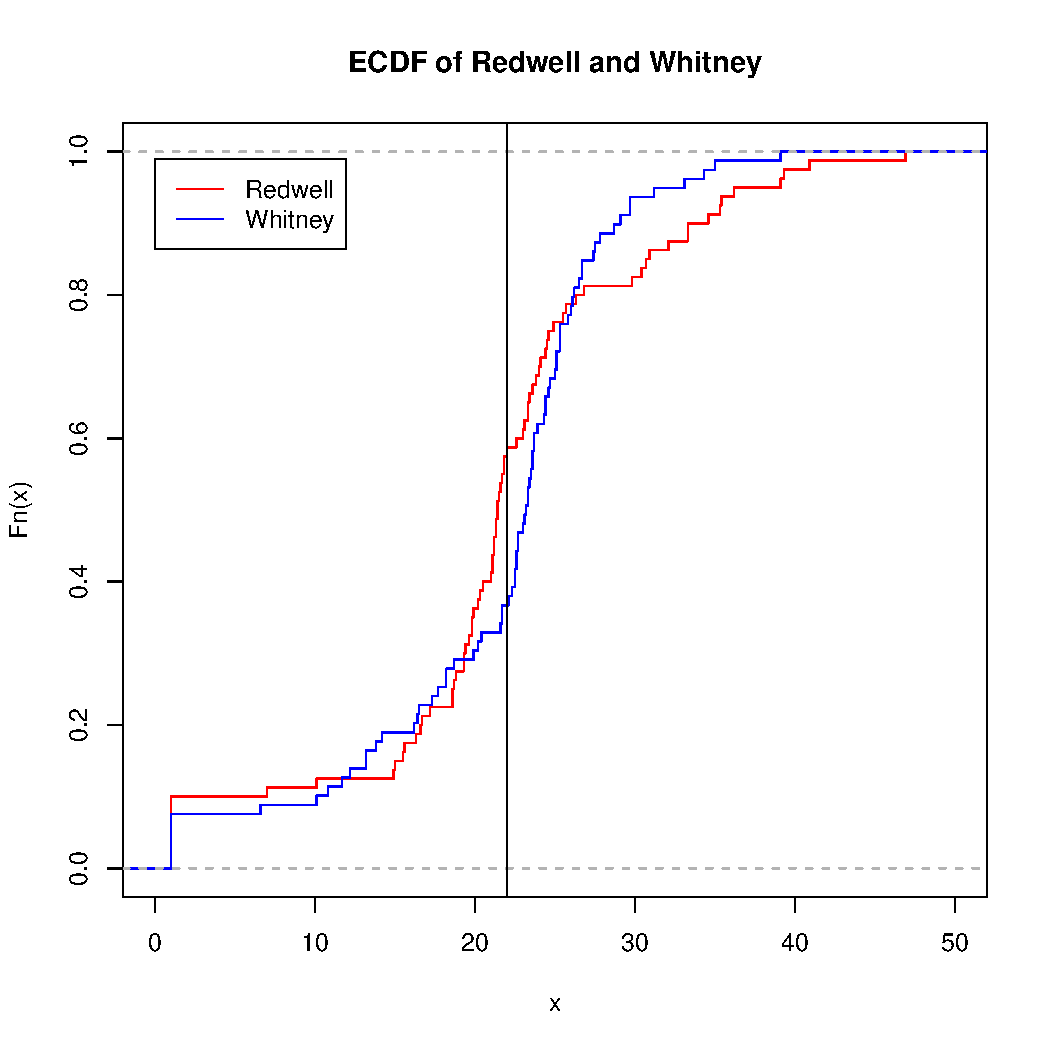
\includegraphics[scale = 0.4]{ex2.pdf}\\
D = 0.2204114
\end{center}
}

\frame{
\frametitle{Example: Two Sample KS test}
In this example, we generate two vectors of random normal variables, where the first vector is based on the standard normal distribution and the second vector is based on the $N(0, 3)$

\texttt{ }\\
\texttt{rnorm1 = rnorm(100, mean = 0, sd = 1)}\\
\texttt{rnorm2 = rnorm(100, mean = 0, sd = 3)}\\
\texttt{t.test(rnorm1, rnorm2)}\\
\texttt{	Welch Two Sample t-test}\\
\texttt{data:  rnorm1 and rnorm2 }\\
\texttt{t = -0.6139, df = 121.777, p-value = 0.5405}\\
\texttt{alternative hypothesis: true difference in means is not equal to 0}\\
\texttt{95 percent confidence interval:}\\
\texttt{ -0.8262021  0.4350894 }\\
\texttt{sample estimates:}\\
\texttt{mean of x mean of y}\\ 
\texttt{0.1094451 0.3050015}
}

\frame{
\frametitle{Example: Two Sample KS Test}
We see that the $t$-test does not pick up on the difference of the populations because the means are, in fact, the same in the two population distributions.  However, the KS test picks up on the difference between the two distributions:

\texttt{ }\\
\texttt{ks.test(rnorm1, rnorm2)}\\

\texttt{	Two-sample Kolmogorov-Smirnov test}\\
\texttt{data:  rnorm1 and rnorm2 }\\
\texttt{D = 0.29, p-value = 0.0004453}\\
\texttt{alternative hypothesis: two-sided} \\
\texttt{}\\

Note: We can also use the function qqstats:

\texttt{qqstats(rnorm1, rnorm2)\$maxdiff \# 0.29}
}

\frame{
\begin{center}
\frametitle{Example: Two Sample KS Test}
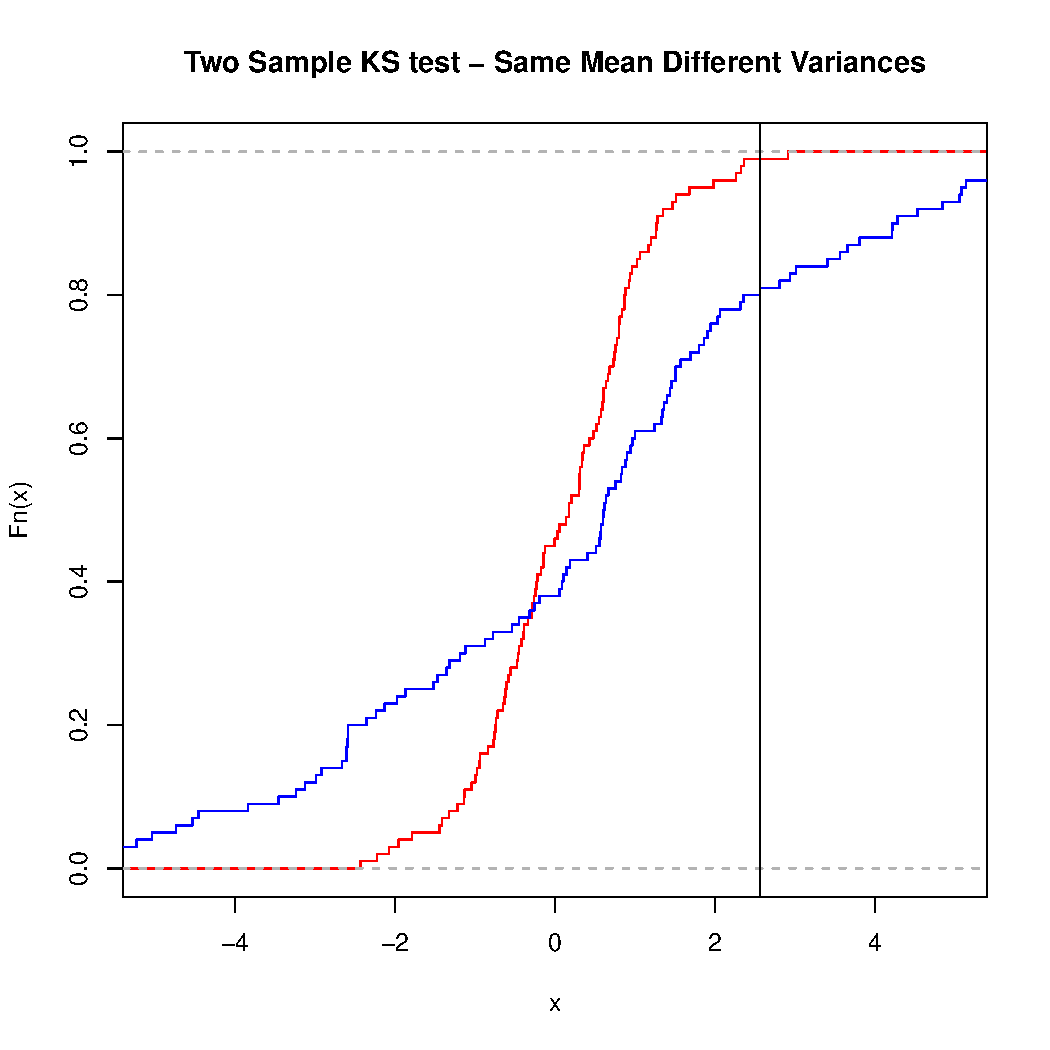
\includegraphics[scale = 0.4]{ex3.pdf}\\
D = 0.29
\end{center}
}

\frame{
\frametitle{Final Notes}
\begin{itemize}
\item The crucial feature of the KS test is that it is distribution free for any continuous common population distribution, because order is preserved under monotone transformations.
\item Another way to see this is to note that the KS test is a \emph{rank} test, because the statistic $D_{m, n}$ depends only on the rank of the observations and not their actual values
\item The rank of the two groups of observations determine the relative positions of the steps of the two graphs of the empirical distribution functions
\item The standard KS test does not provide the correct p-value for non-continuous variables, but the bootstrapped KS does provide the correct p-values.
\item The KS test isn't very powerful, so for example, if you do have normally distributed data and want to do a test for difference in means, t-test would be more powerful.
\end{itemize}
}

\end{document}